\documentclass[11pt,a4paper]{article}
\usepackage{fullpage}
\usepackage{amsmath}
\usepackage{amssymb}
\usepackage{amsfonts}
\usepackage{mathtools}
\usepackage{titlesec}
\usepackage{graphicx}
\usepackage{float}
\usepackage{wrapfig}
\usepackage{multicol}
\usepackage{caption}
\usepackage{hyperref}
\usepackage{apacite}
\usepackage{multirow}
\usepackage{subcaption}
\captionsetup{justification=centering}
\titleformat*{\section}{\large\bfseries}
\usepackage[table]{xcolor}
\usepackage{graphicx}
\usepackage{array}

    \makeatletter
\newcommand{\thickhline}{%
	\noalign {\ifnum 0=`}\fi \hrule height 1pt
	\futurelet \reserved@a \@xhline
}
\newcolumntype{"}{@{\vrule width 1pt}}
\makeatother



\begin{document}
	
	\title{\textbf{Master Project \\ Computer Graphics: Rendering Track}}
	\author{\textbf{Alhajras Algdairy} \\ \textbf{Advisor: Prof. 
			Dr.-Ing. Matthias Teschner}}
	\maketitle
	
	\section*{\centering Acknowledgment}
	I want to express my special thanks of gratitude to Prof. Dr.-Ing. Matthias Teschner, who guided me through my master's program in general and in this master's project in specific. This project gave me the golden opportunity to dig into an exciting topic in computer graphics that I am keen on. The flexibility in research made me learn more about the related topics I am interested in, in rendering. Reading scientific topics and reviewing codes from different repositories expanded my expertise, where I had a full responsibility to control my time and resources, to learn more about the research process. 	
	
	\section*{\centering Abstract}
	This report investigates four different acceleration data-structure methods for implementing a simple raytracer on CPU. These methods are KD-tree, Uniformgrid, BVH, and LBVH. The report aims to compare the different approaches and their impact on the raytracer rendering time. The raytracer used in this project builds upon a previous lab project where the foundation of the raytracer is already implemented; however, without using a sophisticated data-structure to enhance the rending performance; hence the focus of this report will be how to improve the raytracer performance by using data-structures. 
	\textbf{\textit{Keywords: Ray Tracing; kD-Tree; BVH; LBVH; Uniformgird; Data structure;}}
	
	\section{Introduction}
	This report summarises my journey to implement a simple raytracer focusing on data structure level, where the performance of rending a scene will be the lion's share of the report. Theory, implementation, and results will be discussed in depth in the report, where an introduction and motivation of what is raytracer and how to implement it will be briefly discussed; because data structures are more interesting for us, I will only explain the topics that are used in this raytracer. 
	
	\section{What is Raytrcer and how it works}
	
	Computer graphics has three main pillars: \textit{Modelling}, \textit{Rendering}, and \textit{Simulation}. Scientists are interested in simulating a real-life phenomenon, such as Gravity Fraction, Rain, Snow, and the exciting part for us, light.  Simulating light is arguably the most challenging part because light has always been difficult to characterize as it can behave as particles and waves, which makes it spread into the whole scene based on probabilities. This makes it difficult to compute as it involves complex computation and infinite simulations to execute to have a perfect result without an error, this is what is known as Rendering.
	
	Why do we need to simulate light? Adding light into a scene will generate shadows, reflection, and refraction consequently will illuminate the scene, making the scene look like a reality, which can be helpful for some applications. For the internal designers, it is vital to simulate the final result of the lightning inside a room, such as sunlight coming from the windows, the light of lamps, and fireplace, these with react together and create shadows, before constructing the building and payloads of money, simulating the right angle and place of the room is helpful to imagine the final result. Solar engineers use 3D tools to build solar panel farms where the angle between the sunlight and the panel is essential to gather as much light energy as possible. In gaming, different companies compete to design engines that can produce natural scenes; this includes lighting and shadowing.  
	
	Figure~\ref{fig:1}, shows an example of rending a scene that can not be distinguished from reality, the details it catches as glossy materials, the reflection of surfaces, and the shadow. Capturing these details requires rendering techniques. Two popular methods are Rasterization and Raytracing. Raytracing outperforms rasterization in capturing more details; however this leads to performance issues, that is why most application uses Raytracing is offline rendering and not real-time rendering like games, where speed is vital to render each frame with compromising details. 
	
	
		\begin{figure}[H]
		\begin{center}
		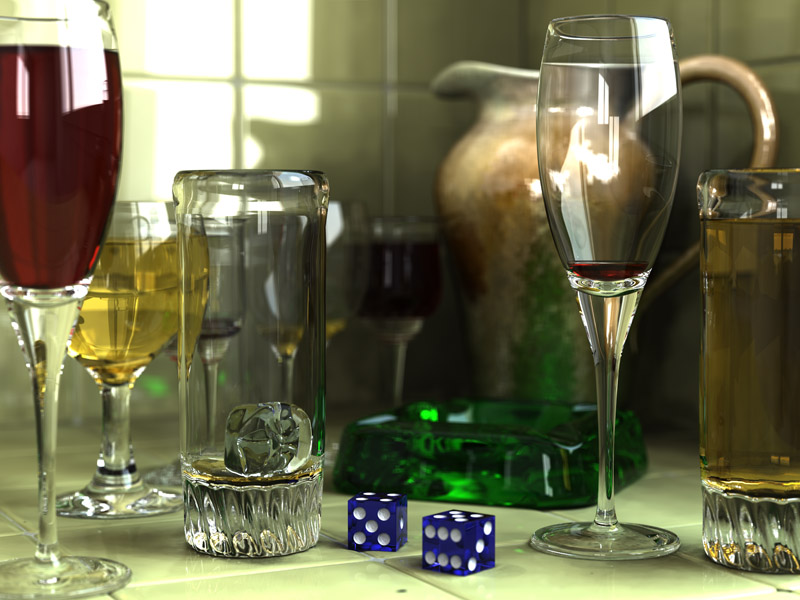
\includegraphics[width=0.7\textwidth]{1.jpg}
			
			\caption{https://www.pcgamer.com/unreal-engine-5-tech-demo-pc-performance/ The raytracing algorithm builds an image by extending rays into a scene and bouncing them off surfaces and towards sources of light to approximate the color value of pixels [Piotr Dubla, "Interactive Global Illumination on the CPU."
				]}
			\label{fig:1}
		\end{center}
	\end{figure}

		
	\subsection{Raytracing definition}
	So what is Raytracing? Raytracing is a rendering technique that provides highly lifelike lighting effects. In other words, an algorithm can track the source of light and then mimic how the light interacts with the virtual objects it eventually encounters in the computer-generated environment. Raytracing produces far more lifelike shadows and reflections, as well as significantly enhanced translucence and dispersion. The algorithm considers where the light falls and calculates the interaction and interplay in the same way as the human eye does with actual light, shadows, and reflections.
	
	\vspace*{5px}
	
	\subsection{Raytracing mechanism}
	Raytracing follows three main steps: 
	\textit{Casting Rays}: This is similar to how the eye works, however rather than eyes works as a sensor, we have a camera, we shoot rays from the camera to the scene, and we calculate which is the closest object it hits, its color and brightness. This is done for each pixel.
	\textit{Path tracing}: Casting rays can solve the visibility issue; this means which object appears on the camera and at what position and color. However, if we want to simulate the following effects:  soft shadows, depth of field, motion blur, caustics, ambient occlusion, and indirect lighting, then we need to trace the rays from or to the light source, this will accumulate the brightness of an object or model in a scene, also will give the depth of different objects. Note that the more rays and depth we need, the more quality we get but the slow the simulation becomes due to the complexity.
	\textit{Shading}: In addition to tracing rays, we need a model to simulate different materials like Transparent, Glossy, and Diffuse. This is where the Shading phase is needed.
	
	\vspace*{5px}
	Raytracing has two main methods: 
	\begin{itemize}
		\item 		\textit{Forward Raytracing}: The light particles (photons) are tracked from the light source to the object via Forward Raytracing. While forward ray tracing is the most exact method for determining the color of each object, it is also the most inefficient.
		\item 		\textit{Backward Raytracing}: 
		An eye ray is formed at the eye in backward ray tracing, and it travels through the viewplane and out into the scene. If it hits an object, it will return it to the viewplane immediately. This method is more efficient than Forward Raytracing but less accurate due to reducing the rays used. In this implementation this method is used.
	\end{itemize}
	
	\section{Raytracer Implementation}
	In this chapter, raytracer terms and definitions are introduced, illustrating the implementation and decisions that have been made. 
	We need to set up our implementation to work for the raytracer as shown in Figure 2; the basic raytracer requires a camera; its responsibility is to shoot rays that travel through the scene and return a value or color. How many rays should it shoot? This depends on the width and height of the image we want to generate, the bigger the image, the more details we capture, but the more expensive computation gets. The rays idea is to find an intersection with the scene objects and try to return a color of the object to represent a corresponding pixel value. For object visibilities, we do not need a light source; however, to make the scene more realistic, we need to add shadows and other effects as reflections and refractions; hence we need a source light and tools, as shown in Figure 2.
	
	The algorithm works as follows, initiating the camera position and the orientation direction or where it looks at. Secondly, we subdivide the scene into pixels; this is based on the settings of the raytracer, usually by setting a height and width, reading a scene from usually an XML file that has a description of the number of objects in the scene, their color, and type. Afterward, generating rays for each pixel, this ray will be shooted toward the scene, and for each ray, we go through all the objects and test intersection tests; if the test returns true, we save its position, and we save the object, we do this for all objects and if more than two objects are intersected we compare between their position to detect which one is closer to the camera. In order to create shadows, we track the intersection point from the camera toward the light; if there is an object between the light source the hitting point, then we detect shadow. The corresponding value of the pixel is saved in a buffer and after the ray tracing is done, the pixels value are saved in a file of PPM extention.
	
	This is the basic idea, and to improve it, other topics need to be covered, such as Data structures, Objects Materials, Anti aliasing, Soft shadow. In this chapter, the basic blocks and components that make up the raytracer will be explained; only the methods are used will be explained, because as mentioned before, the performance of the raytracer is the main scope for this project.
	 
	 	 	
	 \begin{figure}[H]	
	 	\begin{center}
	 		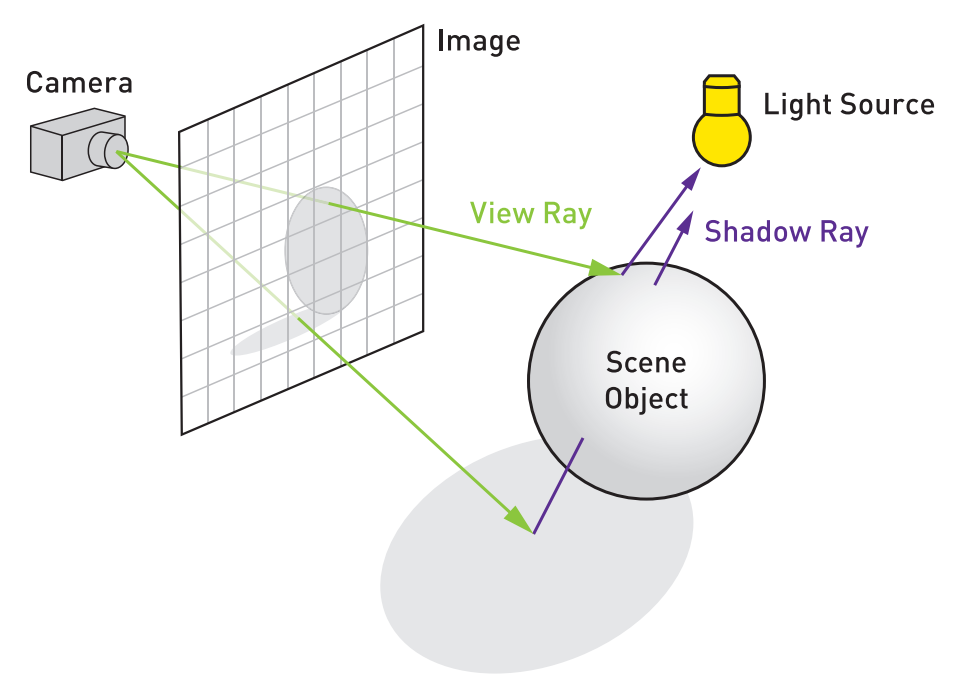
\includegraphics[width=0.7\textwidth]{4.png}
	 		
	 		\caption{ An image showing how a ray is casted from the camera and how objects are illuminated and shadows are computed in ray tracing	.} %\protect\cite{haines2019ray}%
	 		\label{fig:1}
	 	\end{center}
	 \end{figure}
 
	\subsection{Software architecture}
	\subsubsection*{Configuration}
	We start with the configuration of the Raytracer by introducing a \textbf{struct Settings}, here we specify the following properties of the raytracer such as the \textbf{width} of the image, \textbf{height} of the image, the \textbf{background default color} of the scene, \textbf{maximum depth of path tracing},  \textbf{anti-aliasing samples} and \textbf{acceleration data Structure type}. Some of the previous terms will be explained later. 


	\subsubsection*{Scene generation}
	To create a scene, spheres will be used to create meshes; mesh is a collection of objects at a position and orientation to build a much more complex object. For example, the Stanford bunny shown in Figure 3 is composed of approximately 35947 spheres. Usually, meshes are made of triangles because they are more efficient and easier to build a mesh; however, I want to try to use something else and test the result and the quality of spheres. \textbf{createScene()} is implemented to load .obj files the next models will be used for testing in this report: \textbf{Stanford Bunny}, \textbf{Igea} and \textbf{Armadillo}, Figure 4 shows the different complex model that will be used for testing.

	 \begin{figure}[H]
	\begin{center}
	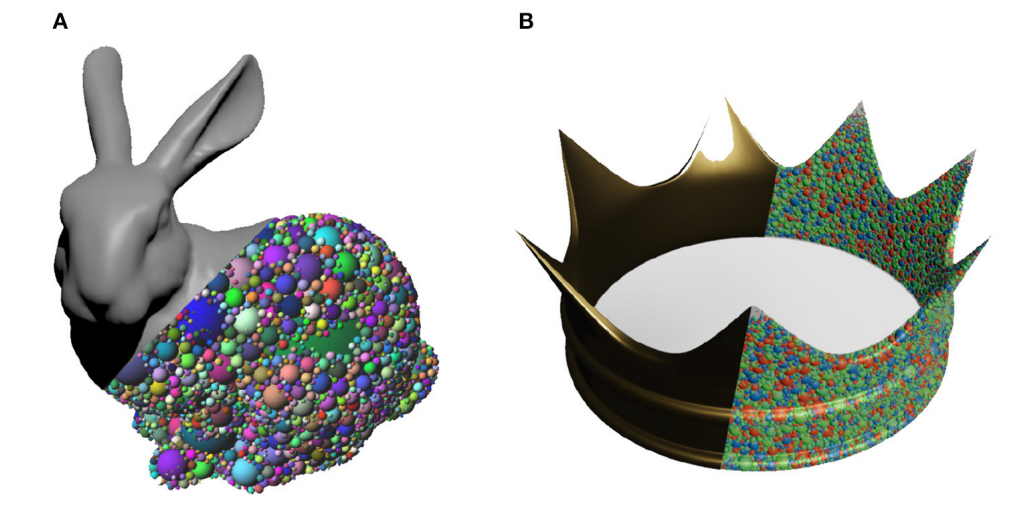
\includegraphics[width=0.7\textwidth]{5.PNG}
	
	\caption{ Stanford bunny and a crown made of a collection od spheres	.}
	 %UnrealHaptics: Plugins for Advanced VR Interactions in Modern Game Engines%
	\label{fig:2}
	\end{center}
	\end{figure}

	\begin{figure}[ht]
	\begin{center}
		\begin{subfigure}{.3\textwidth}
			\centering
			% include first image
			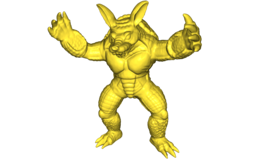
\includegraphics[width=.8\linewidth]{armadillo.png}  
			\caption{Armadillo model}
			\label{fig:sub-first}
		\end{subfigure}
		\begin{subfigure}{.3\textwidth}
			\centering
			% include second image
			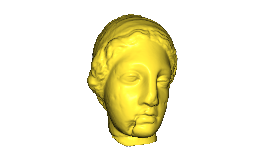
\includegraphics[width=.8\linewidth]{igea.png}  
			\caption{Igea model}
			\label{fig:sub-second}
		\end{subfigure}
		\begin{subfigure}{.3\textwidth}
			\centering
			% include second image
			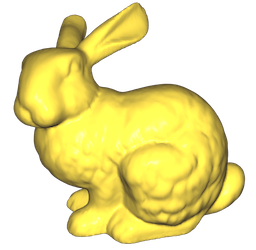
\includegraphics[width=.8\linewidth]{stanford-bunny.png}  
			\caption{Stanford-bunny model}
			\label{fig:sub-third}
		\end{subfigure}
		
		\caption{Rendering different shapes in the scene}
		\label{fig:5}
		
	\end{center}
\end{figure}

    The \textbf{Sphere} is a class with the next attributes: \textbf{Center}: Position of the sphere, \textbf{MaterialType}: \textit{diffuse}, \textit{glossy}, \textit{reflection} and \textit{refraction} ,\textbf{Radius}: Sphere radius usually 1, \textbf{surfaceColor}: Color of the sphere in \textbf{RGB} format, and \textbf{emissionColor}: This is for the light.   
	Lights are just vector of spheres where the \textbf{emissionColor} is set to one. The light emeission is using the \textbf{inverse-square law}. In science, an inverse-square law is any scientific law stating that a specified physical quantity is inversely proportional to the square of the distance from the source of that physical quantity. In other words, the more significant the distance between the light source and the object, the less light it reaches the object surface.
	
		\noindent For point lights, this can be formulated as:
	\begin{equation}
		l_{ip} = \frac{l_{i}}{4 * \pi * d^2}
	\end{equation}
	where $l_{ip}$ is the actual intensity reaching a point $\boldsymbol{p}$, $l_{i}$ is the intensity value of the light and $d$ is the distance between the light position $\boldsymbol{l}_{p}$ and point $\boldsymbol{p}$.
	\subsubsection*{Shooting rays}
		For this, all raytracers use rays as a way to simulate photons. Let us think of a ray as a function; here $\pmb{p} $ is a 3D position along a line in 3D. $\pmb{o} $ is the ray origin and $\pmb{d} $ is the ray direction.
	\begin{equation}
		\pmb{p} (t) = \pmb{o} + t\pmb{d} ,  \quad  0 < t < \infty
	\end{equation}
	
	Figure 5 shows how Rays are used and how equations 1 can be used to check intersection tests and calculate the distance between the origin ray point, the camera, and the intersection point.  Point distance $\pmb{d} $ is used to compare the points to check which object is closer to the camera. 
	
			 \begin{figure}[H]	
			\begin{center}
				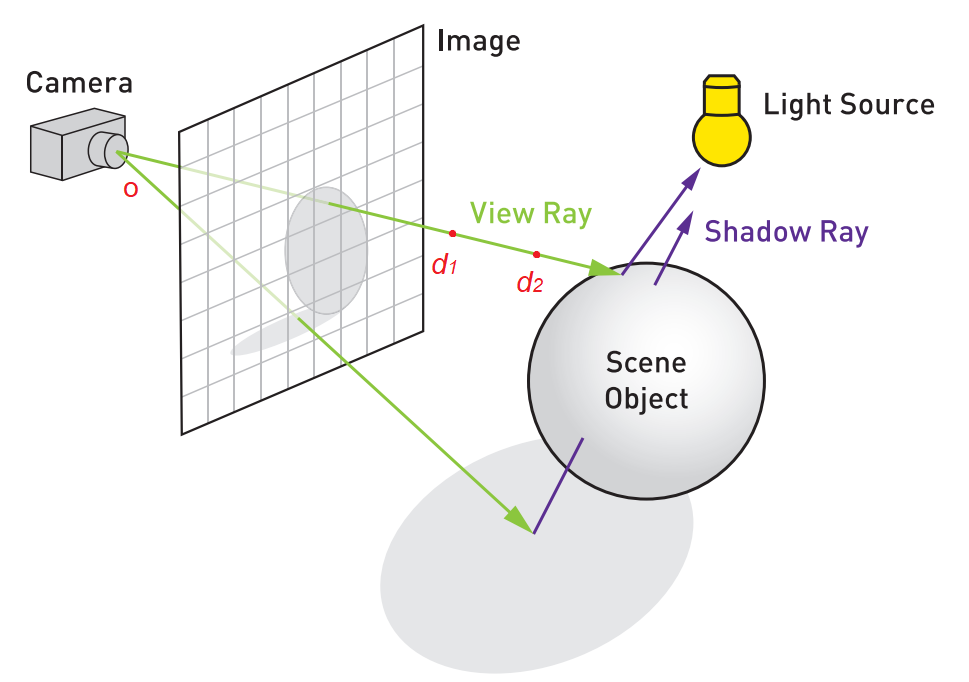
\includegraphics[width=0.7\textwidth]{6.png}
				
				\caption{ An image showing how a ray is casted from the camera and how objects are illuminated and shadows are computed in ray tracing	.} %\protect\cite{haines2019ray}%
				\label{fig:1}
			\end{center}
		\end{figure}
	
	\subsubsection*{Rendering Sphere}
	For testing, spheres are often used in ray tracers because
	calculating whether a ray hits a sphere is pretty straightforward.
	
	The general equation of a sphere with radius = 1 is:
	\begin{equation}
		(o_x + td_x )^2 + (o_y + td_y )^2+ (o_z + td_z )^2= 1
	\end{equation}
	
	For solving the equation we need to use the Quadratic equation in $ t $: 
	
	\begin{equation}
		\begin{split}
			A(t)^2 + Bt+ C= 0 \\
			A = d^2_x + d^2_y + d^2_z \\	
			B = 2(d_xo_x + d_yo_y + d_zo_z) \\
			C = o^2_x + o^2_y + o^2_z - 1 \\
			t_{1,2} = \frac{-B \pm \sqrt{B^2 - 4AC}}{2A}\\
		\end{split}		
	\end{equation}
	
	
	By solving the equation we get three different cases as shown in Figure ~\ref{fig:2}:
	
	\begin{itemize}
		\item No Intersection if: \( B^2 - 4AC < 0 \) 
		\item Single point of intersection if: \( B^2 - 4AC = 0 \)
		\item Otherwise we get two points of intersection
	\end{itemize}
	
	
	\begin{figure}[H]
		\begin{center}
			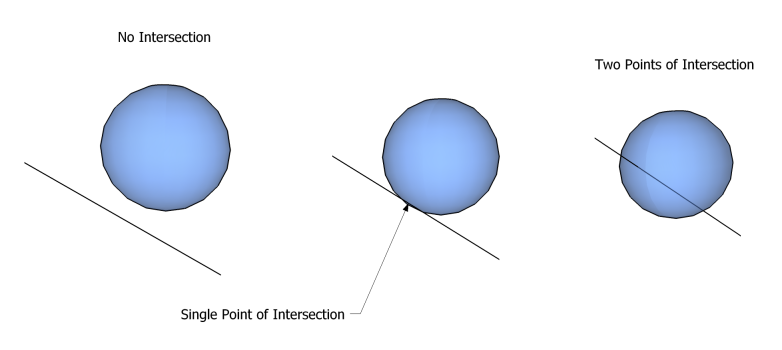
\includegraphics[width=250pt]{C:/D/University/Semester_4/Raytracer/lab_report_1/assignment_2/images/5.png}
			
			\caption{The three possible line-sphere intersections:
				1. No intersection.
				2. Single point intersection.
				3. Two point intersection.}
			\label{fig:2}
		\end{center}
	\end{figure}
	
	\subsubsection*{Shading}
	The second step in rendering a scene is \textit{Shading}, and this deals with the color of the object and its intensity. Shading also includes how object's color affects each other; for example, having light hits, the object will make its color look brighter; on the other hand, regions in which light does not hit or reach will have dark color or shadow. In this chapter, shading concepts will be discussed and implemented, in addition to different materials that have different properties and how they interact with the light. The primary key to Shading is calculating the amount of light that hits a point; let us call it $ P $. 
	
	The computed light at a point $ P $ depends on the following: 
	
	\begin{itemize}
		\item Light illuminated by source  $\pmb{L}^{source}$  in real life usually lamp, fire or the sun, it can have any color and intensity but here we will use white color. 
		\item Surface illumination $\pmb{L}^{surface}$.
		\item Light reflected from the surface $\pmb{L}^{reflected}$.
		\item The observation angle / looking at angle / camera. 
	\end{itemize}
	
	
	
	
	\subsubsection{Lambert's Cosine Law}
	The amount of light energy arriving at a surface is proportional to the cosine of the angle between the light direction and the surface normal, according to \textit{Lambert's cosine law}. Illumination strength at a surface is proportional to the cosine of the angle between $\pmb{l}$ and $\pmb{n}$, the angel will be denoted as $\theta$, the following three cases illustrate the relationship between the  $\pmb{L}^{source}$ and  $\pmb{L}^{surface}$:
	
	The  $\pmb{L}^{surface}$,$ \pmb{L}^{source}$ relation is:
	
	\begin{equation}
		\pmb{L}^{surface} = \pmb{L}^{source}.\cos \theta 
	\end{equation}
	
	
	\begin{itemize}
		\item $\pmb{L}^{surface} = \pmb{L}^{source}$, if $\theta = 0\degree$.
		\item $\pmb{L}^{surface} = 0$, if $\theta = 90\degree$.
		\item $0 < \pmb{L}^{surface} < \pmb{L}^{source}$, if $0\degree < \theta  < 90\degree$.
	\end{itemize}
	
	\subsubsection{Phong reflection model }
	Phong reflection is a model of local illumination. It defines how light reflects off a surface as a mixture of \textit{diffuse} reflection from rough surfaces and \textit{specular} reflection from polished surfaces. It's based on Phong's intuitive observation that bright surfaces have small, strong specular highlights, and dull surfaces have larger, more gradual specular highlights. The model also includes an ambient term to account for the small amount of light that is scattered about the entire scene.
	\\
	
	\begin{itemize}
		\item \pmb{Ambient reflection}
		\begin{equation}
			\pmb{L}^{amb} = \pmb{\rho}\otimes \pmb{L}^{indirect}
		\end{equation}
		
		\begin{itemize}
			\item $\pmb{\rho}$, is the surface color
			\item $\pmb{L}^{indirect}$ , is the light reflected from other surfaces and objects, excluded the direct light ($\pmb{L}^{source}$)
		\end{itemize}
		\item \pmb{Diffuse reflection} 
		
		\begin{equation}
			\pmb{L}^{diff} =  \pmb{L}^{source}.(\pmb{n}.\pmb{l}) \otimes \pmb{\rho} 
		\end{equation}
		\begin{itemize}
			\item $\pmb{L}^{source}$, is the light source color and intensity which usually white. 
			\item $\pmb{n}$ and $\pmb{l}$ , are the representation of the Lambert's cosine law, where $\pmb{n}$ is the normal surface vector  and $\pmb{l}$ is the indecent light coming from the light source.
		\end{itemize}
		\item \pmb{Specular reflection} 
		
		\begin{equation}
			\pmb{L}^{spec} =  \pmb{L}^{source}.(\pmb{n}.\pmb{l}).(\pmb{r}.\pmb{v})^m \otimes \pmb{\rho}^{white} 
		\end{equation}
		\begin{itemize}
			\item $\pmb{r}$, which is the direction that a perfectly reflected ray of light would take from this point on the surface. 
			\item $\pmb{v}$, which is the direction pointing towards the viewer (such as a virtual camera).
			\item $m$, which is a shininess constant for this material, which is larger for surfaces that are smoother and more mirror-like. When this constant is large the specular highlight is small.
		\end{itemize}
	\end{itemize}
	
	The overall illumination on the surface can be computed by summing up the three components that make up \textit{Phong model}:
	
	\begin{equation}
		\pmb{L}^{surface}= \pmb{L}^{amb} + \sum_{n=1}^{lights} (\pmb{L}_n^{diff} + \pmb{L}_n^{spec})
	\end{equation}
	
	
	\begin{figure}[ht]
		\begin{center}
			\begin{subfigure}{.3\textwidth}
				\centering
				% include first image
				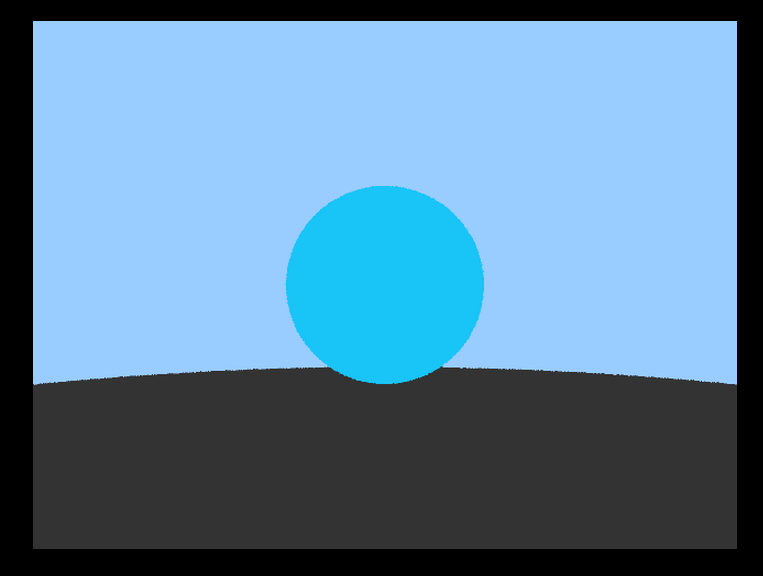
\includegraphics[width=.8\linewidth]{C:/D/University/Semester_4/Raytracer/lab_report_1/assignment_2/images/amb_reflection.png}  
				\caption{Ambient $ \pmb{L}^{amb} $}
				\label{fig:sub-first}
			\end{subfigure}
			\begin{subfigure}{.3\textwidth}
				\centering
				% include second image
				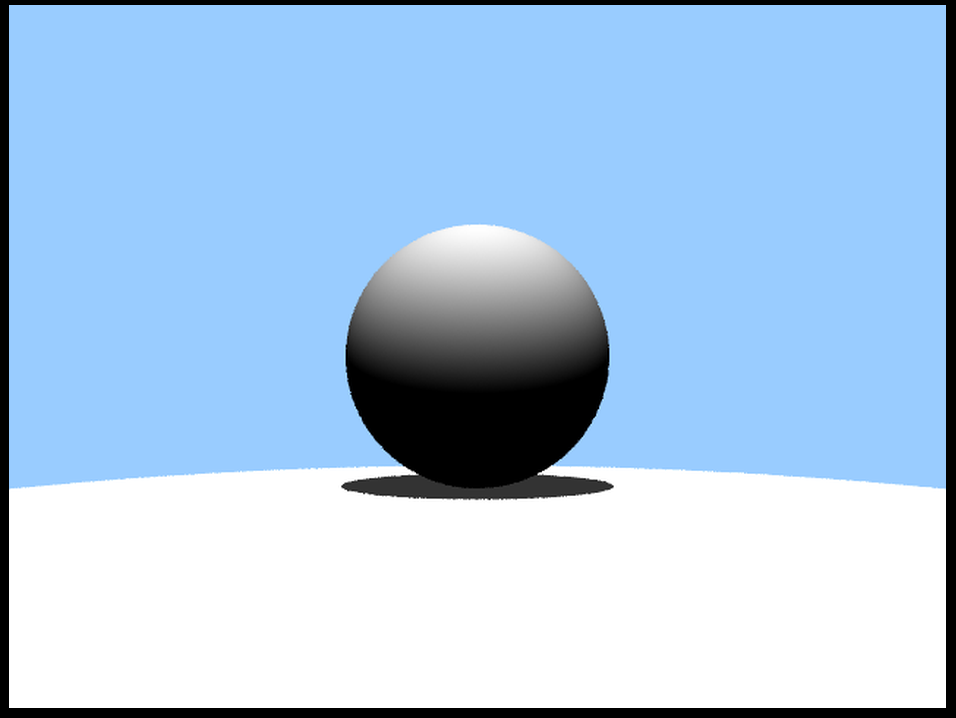
\includegraphics[width=.8\linewidth]{C:/D/University/Semester_4/Raytracer/lab_report_1/assignment_2/images/diff_reflection_2.png}  
				\caption{Diffuse $ \pmb{L}^{diff} $}
				\label{fig:sub-second}
			\end{subfigure}
			\begin{subfigure}{.3\textwidth}
				\centering
				% include second image
				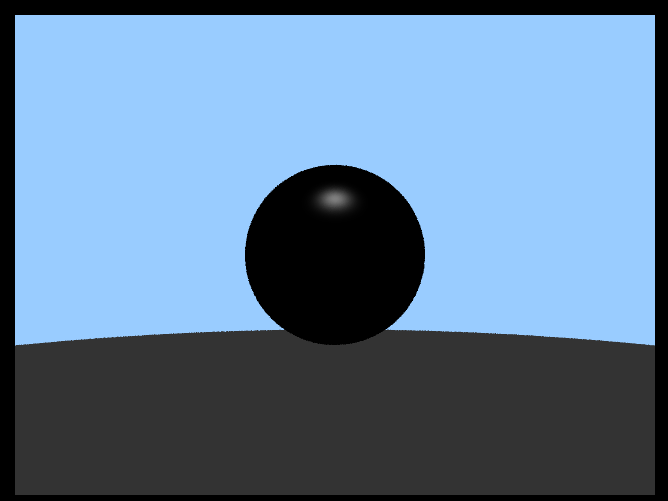
\includegraphics[width=.8\linewidth]{C:/D/University/Semester_4/Raytracer/lab_report_1/assignment_2/images/spec_reflection_2.png}  
				\caption{ Specular (Glossy)  $ \pmb{L}^{spec} $}
				\label{fig:sub-third}
			\end{subfigure}
			
			\caption{Visual illustration of the Phong equation}
			\label{fig:6}
		\end{center}
	\end{figure}


	\section{Performance}
	This is the most exciting part of the project; the previous chapters explained how to set up the current Raytracer and what methods have been used to implement it; however, the result is not shown yet. This chapter will apply different performance tests on the Raytracer to show its average performance without optimizing the datastrcuter. 
	
	In the renderer the next setup is used: 
	
	\begin{table}[h]
		\centering
		\begin{tabular}{ c|c  }
			\hline
			Key   &   Value \\
			\hline
			Height   &   480 \\
			
			
			Width   & 640 \\
			
			
			DataStructure   & None \\
			
			
			Anti-aliasing samples  & 2 \\
			
			
			PC info  & 	Intel(R) Core(TM) i7-8565U CPU @ 1.80GHz   1.99 GHz  RAM	16.0 GB\\
			\hline
		\end{tabular}
				\caption{The Raytracer settings.}
	\label{table:2}
	\end{table}
 
		\begin{table}[h]
		\centering
		\begin{tabular}{>{\centering\arraybackslash}m{.1\linewidth}|>{\centering\arraybackslash}m{.1\linewidth}|>{\centering\arraybackslash}m{.1\linewidth}|>{\centering\arraybackslash}m{.1\linewidth}|>{\centering\arraybackslash}m{.6\linewidth}}
			\thickhline%\toprule
			   Model   &   Spheres  & Sphere intersection tests  &   Time taken to render  & Result \\
						\thickhline%\toprule
			     Bunny   &
			   35947  & 1841.98m &   104.31 minutes  & 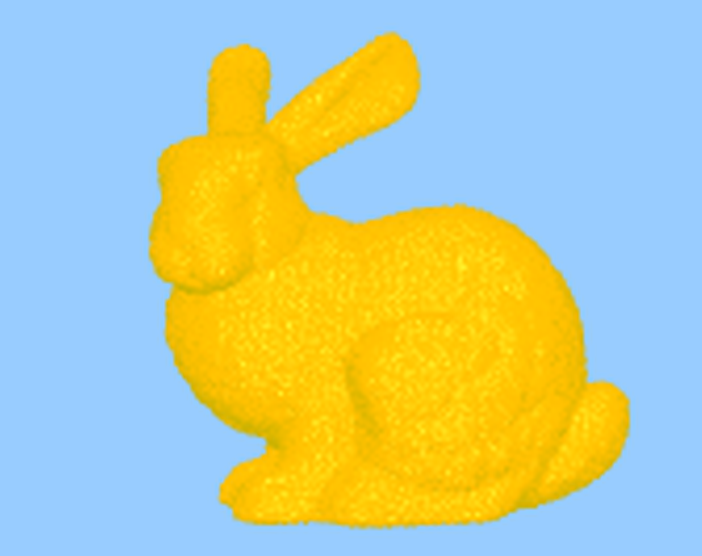
\includegraphics[width=0.3\textwidth, height=50mm]{stanford-bunny_re.PNG}\\
			
			 Armadillo  &   49990    &1822.94m&   45.34 minutes &    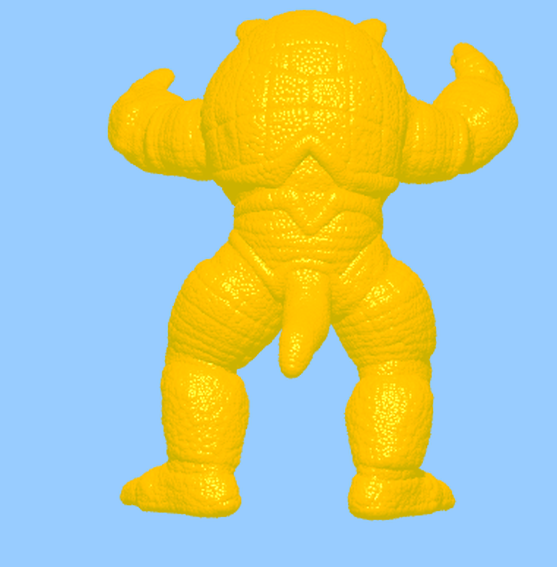
\includegraphics[width=0.3\textwidth, height=50mm]{armadillo_re.PNG} \\
			
			 Igea   &  134345    &7278.88m&   187.5 minutes & 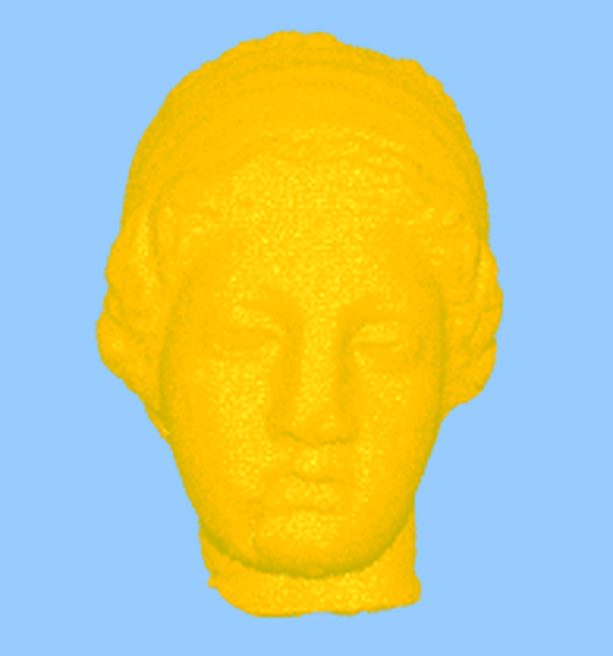
\includegraphics[width=0.3\textwidth, height=50mm]{igea_re.PNG} \\
						\thickhline%\toprule
		\end{tabular}
			\caption{Performance comparison for different scenarios on 480X640.}
	\label{table:2}
	\end{table}


	\section{Object subdivision}
	\section{Spatial Subdivision}
	
	This lab was a great way to gain practical experience of the concepts we learned in our computer graphics course. I would like to thank \textbf{Prof. Dr.-Ing. Matthias Teschner} again for advising me throughout this lab. As a final remark, I would like to mention that I really enjoyed working on area lights. This includes debugging issues as I was working on them as well as how they were fixed. At the end, the results were worth the effort.
	
	\bibliographystyle{apacite}
	\bibliography{References}
	
\end{document}